\section{Orbit Altitude}
\label{mtrOrbAltitude}
During the design of the orbit, very careful attention has to be given to the choice of the mission altitude for the entire formation. This parameter is vital for the lifetime requirement.

Initially it was apparent that the choice of the emitting payload would give a hard altitude constraint, however as described in section (ADD REF TO OPTICAL EMITTING PAYLOAD TRADEOFF HERE), with the use of complex optical instruments it was possible to open a wider range of altitudes for selection. The governing properties of the orbit for altitude selection have now become the orbit perturbations.

This section details the considerations in regards to these properties. A separate radiation exposure analysis is also done. Finally a suitable altitude is chosen based on this analysis.
\subsection{Earth Oblateness}
\label{mtrOrbJ2}
ADD J2 PARAGRAP
\subsection{Perturbations due to Other Celestial Bodies}
\label{mtrOrbSelestialBodies}
ADD MOON PARAGRAPH HERE
\subsection{Solar Radiation Pressure}
\label{mtrOrbSolRadiation}
All orbiting bodies are affected by solar radiation pressure. The acceleration due to this phenomenon can potentially affect stationkeeping of the swarm if all satellites have different cross-sectional areas normal to the sun. This perturbation is not directly related to orbit altitude, however it is an important step in orbit analysis. In figure \ref{fig:solarRadArea} on page \pageref{fig:solarRadArea}, the relationship between the acceleration and the normal area to the sun for different satellite masses is shown. Similarly, a graph relating the mass to the acceleration for different cross-sectional areas is shown in figure \ref{fig:solarRadMass} on page \pageref{fig:solarRadMass}.

\begin{figure}[ht!]
\centering
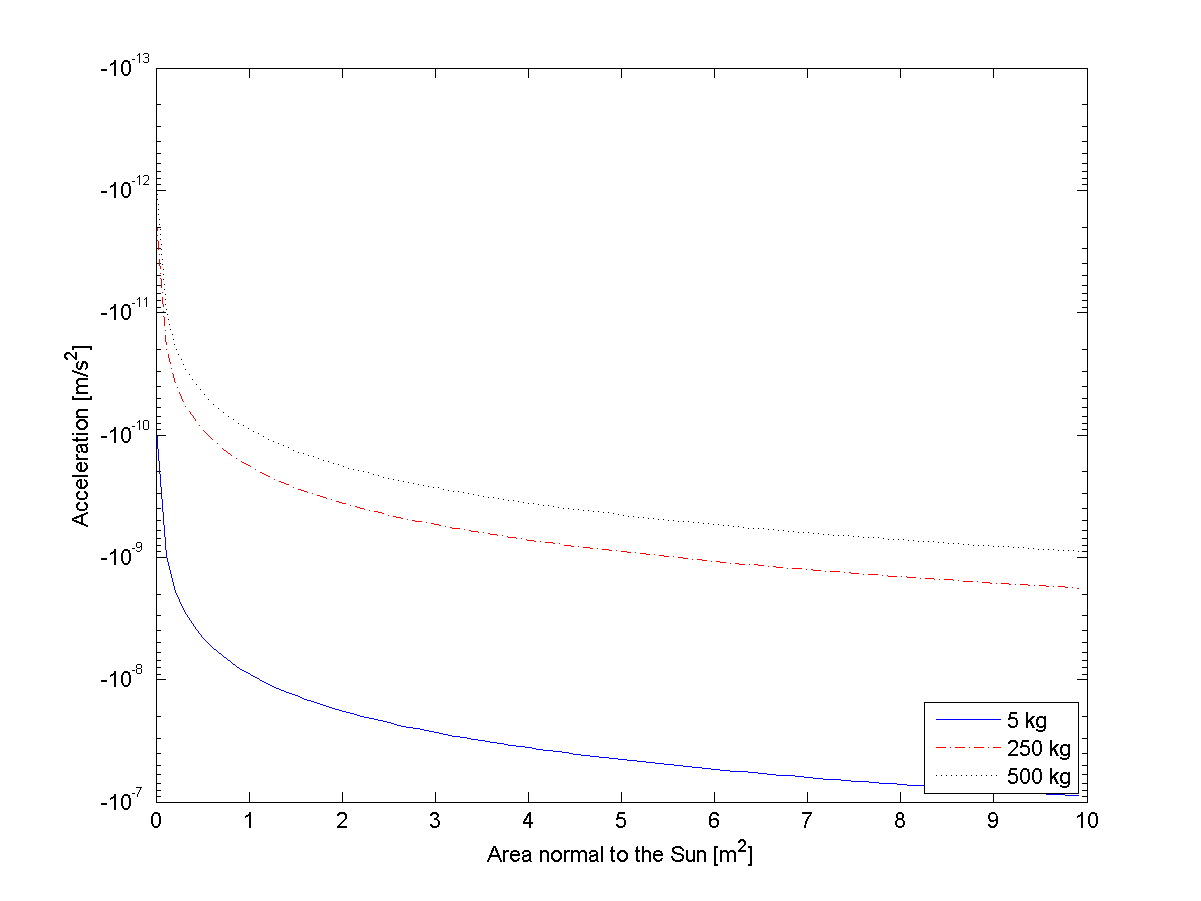
\includegraphics[width=0.8\textwidth, angle=0]{img/solPressureVarArea.png}
\label{fig:solarRadArea}
\caption{Acceleration due to solar radiation pressure vs. area normal to the sun, for different satellite masses.}
\end{figure}

\begin{figure}[ht!]
\centering
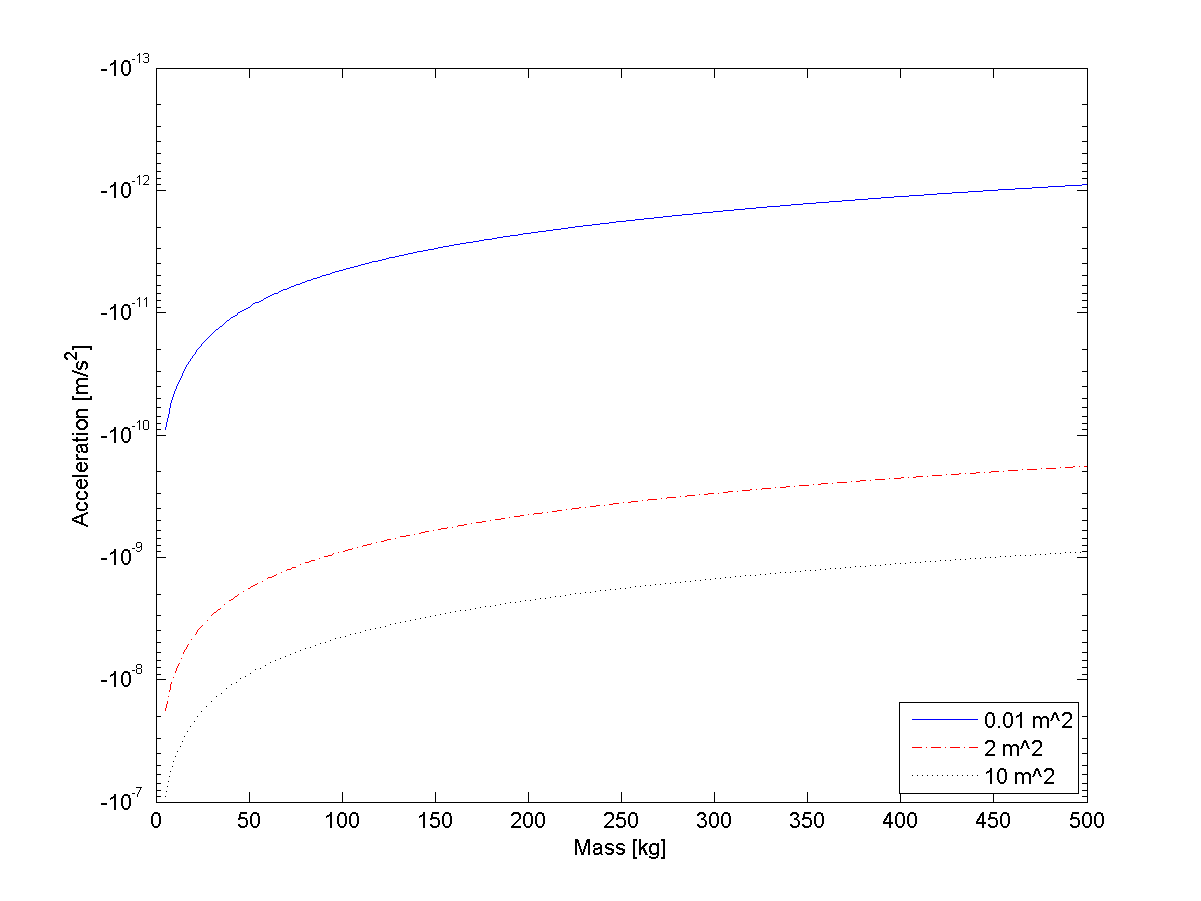
\includegraphics[width=0.8\textwidth, angle=0]{img/solPressureVarMass.png}
\label{fig:solarRadMass}
\caption{Acceleration due to solar radiation pressure vs. mass, for different areas.}
\end{figure}

These figures present design boundary overviews and a general feeling of behavior due to solar radiation pressure is shown. The inverse relationship is obvious. In order to minimize this perturbation it is required to have high mass while retaining the smallest possible area normal to the sun.

What is important to note is that if the ration of area to mass could be maintained constant between the emitting and the receiving satellites, then they would experience the same perturbation, which is a favorable condition. Acceleration with respect to this area/mass ratio can be seen in figure \ref{fig:solarRadRatio} on page \pageref{fig:solarRadRatio}.

\begin{figure}[h!]
\centering
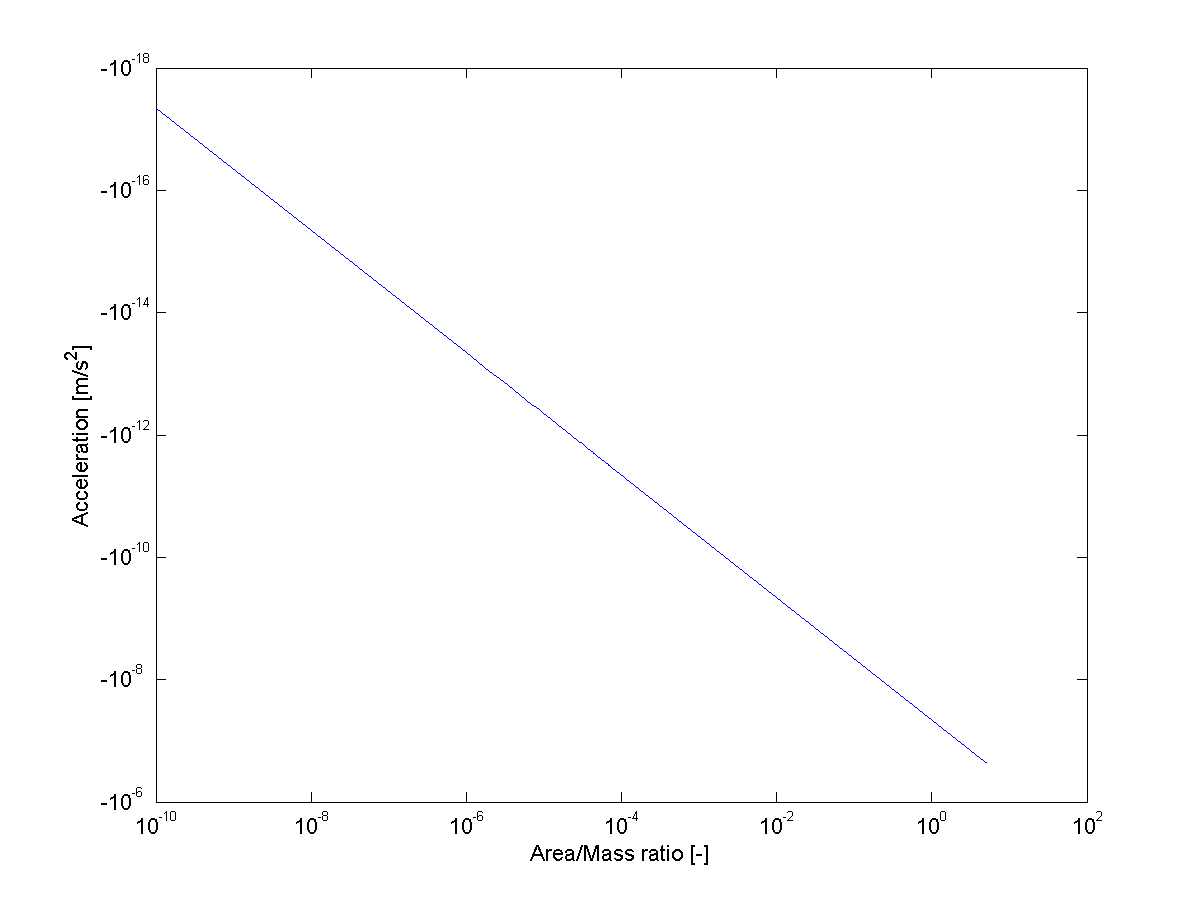
\includegraphics[width=0.8\textwidth, angle=0]{img/solPressureVarRatio.png}
\label{fig:solarRadRatio}
\caption{Acceleration due to solar radiation pressure vs. Area/Mass ratio.}
\end{figure}

\begin{table*}[h]
	\centering
		\begin{tabular}{c|c|c}
		 & Total Mass & Max. Area \\ \hline \hline
		 Emitter & 250 & 10 \\ 
		 Receiver & 50 & 2 
			
		\end{tabular}
	\caption{Mass and area estimates(REVISE)}
	\label{table:solarEstimates}
\end{table*}

Based on preliminary mass and area estimates shown in table \ref{table:solarEstimates} on page \pageref{table:solarEstimates}, it is estimated that the both the emitter and the receiver platforms will experience a decceleration in the order between 10\textsuperscript{-9} and 10\textsuperscript{-10} (CHECK THIS!!). While these values might not seem significant at first, especially relative to atmospheric drag (see section \ref{mtrAtmDrag}), they will become relevant for stationkeeping as explained earlier.

\subsection{Atmospheric Drag}
\label{mtrAtmDrag}

Atmospheric drag is by far the most relevant perturbation for \ac{LEO} satellites. It directly relates to mass as it influences the amount of fuel required to maintain the orbit, where as the mass influences the rate at which the orbit decays. Altitude selection relies heavily on estimation and analysis of drag data as for longer mission times, higher altitudes are preferred, while optical instruments prefer lower altitudes for increased accuracy.

The drag that the satellite experiences due to atmospheric density is described by the following formula:

\begin{equation}
D = -\frac{1}{2} C_D \rho V^2A
\label{drag}
\end{equation}

It follows that orbital parameter changes (semi-major axis, period and velocity respectively) per orbit are calculated using the following equations (assuming negligible eccentricity):

\begin{equation}
\Delta a = -2 \pi \left( C_D \frac{A}{m} \right) \rho a^2
\label{deltaSMA}
\end{equation}
\begin{equation}
\Delta P = -6 \pi \left( C_D \frac{A}{m} \right) \rho \frac{a^2}{V}
\label{deltaP}
\end{equation}
\begin{equation}
\Delta V = \pi \left( C_D \frac{A}{m} \right) \rho aV
\label{deltaV}
\end{equation}

The fundamental problem with accurately predicting effects due to atmospheric drag is twofold: firstly it is very hard to predict the satellite's ballistic coefficient:

\begin{equation}
\frac{m}{AC_D}
\label{ball}
\end{equation}

Even with a well known mass to area ratio, the coefficient of drag can be highly variable, highly dependent on the shape of the satellite and its orientation with respect to the velocity vector. Throughout the following analysis a $C_D$ of 4 has been used as a worst-case scenario. This value is representative of a flat plate traveling with its normal vector pointing in the direction of velocity. In reality this drag coefficient changes. The cross-sectional area normal to the velocity vector can also vary for the swarm satellites if the whole platform is reoriented for instrument pointing. The whole ballistic coefficient ranges from about 25 kgm\textsuperscript{-2} to 100 kgm\textsuperscript{-2}. The satellites being considered in this document are at the lower range of these values.

The second reason drag calculations are so unreliable, is because air density at any altitude is highly variable. Raising air density is primarily connected with solar activity. As solar activity increases every 11 years (see figure \ref{fig:solarCycle} for recorded and predicted solar activity), the atmosphere heats up. Contrary to conventional gas laws that would dictate a fall in density as the gas expands, the atmosphere simply rises, increasing density at higher altitudes.

\begin{figure}[ht!]
\centering
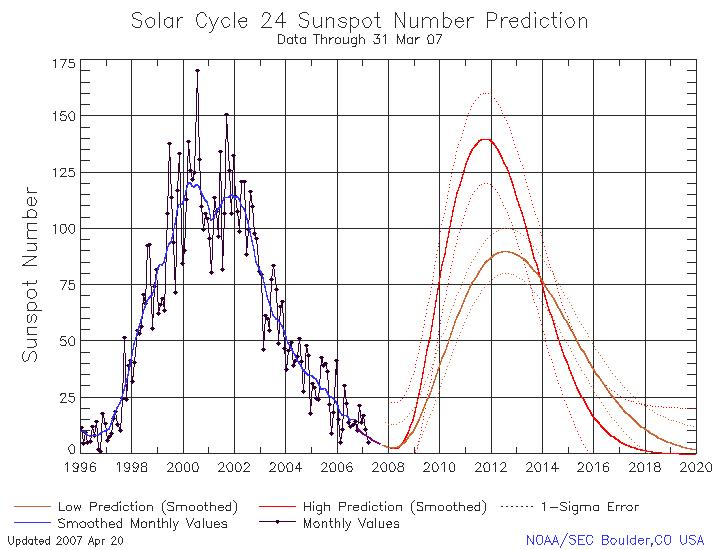
\includegraphics[width=0.9\textwidth, angle=0]{img/solarCycle.jpg}
\label{fig:solarCycle}
\caption{The solar cycle, clearly showing the solar maxima at 11 year intervals. Data after 2007 is projected. \emph{Source: NASA} }
\end{figure}

The density difference during maxima and minima for different altitudes is shown in figure \ref{fig:densityProfile}. Depending on the altitude, the density could vary for up to a whole order of magnitude between the minimum and maximum.

\begin{figure}[ht!]
\centering
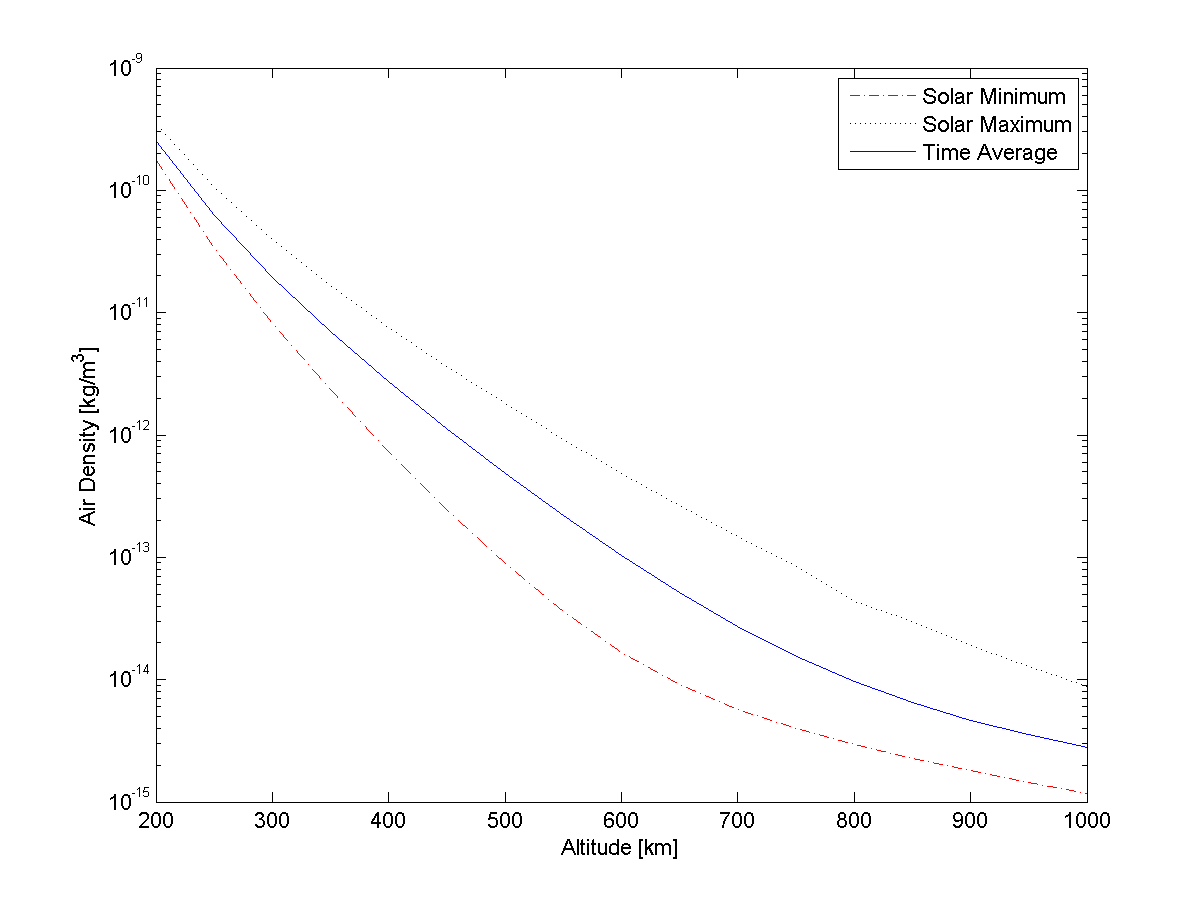
\includegraphics[width=0.9\textwidth, angle=0]{img/densityAltitude.png}
\label{fig:densityProfile}
\caption{Air density vs. orbit altitude for different solar cycle stages.}
\end{figure}

Orbit decay periods for the emitter and receiver satellites are shown in figures \ref{fig:decayEmitter} and \ref{fig:decayReceiver} respectively. The Orbit decay is calculated using equations \ref{deltaSMA} - \ref{deltaV}. Orbit maintenance is not taken into account. The time range considered is a 5 year mission lifetime. The basis for the receiving satellite sizing was taken to be the frontal area of a Delfi-C3 satellite (10x10 cm) plus an initialy estimated solar array area of 0.2 $m^2$. The mass of the said satellite was the same as in table \ref{table:solarEstimates} on page \pageref{table:solarEstimates}. The emitter satellite is sized to be about 0.1 $m^2$ frontal area and an additional 6 $m*2$ of solar array area. The mass is again taken from table \ref{table:solarEstimates} (REVISE!).

\begin{figure}[h!]
\centering
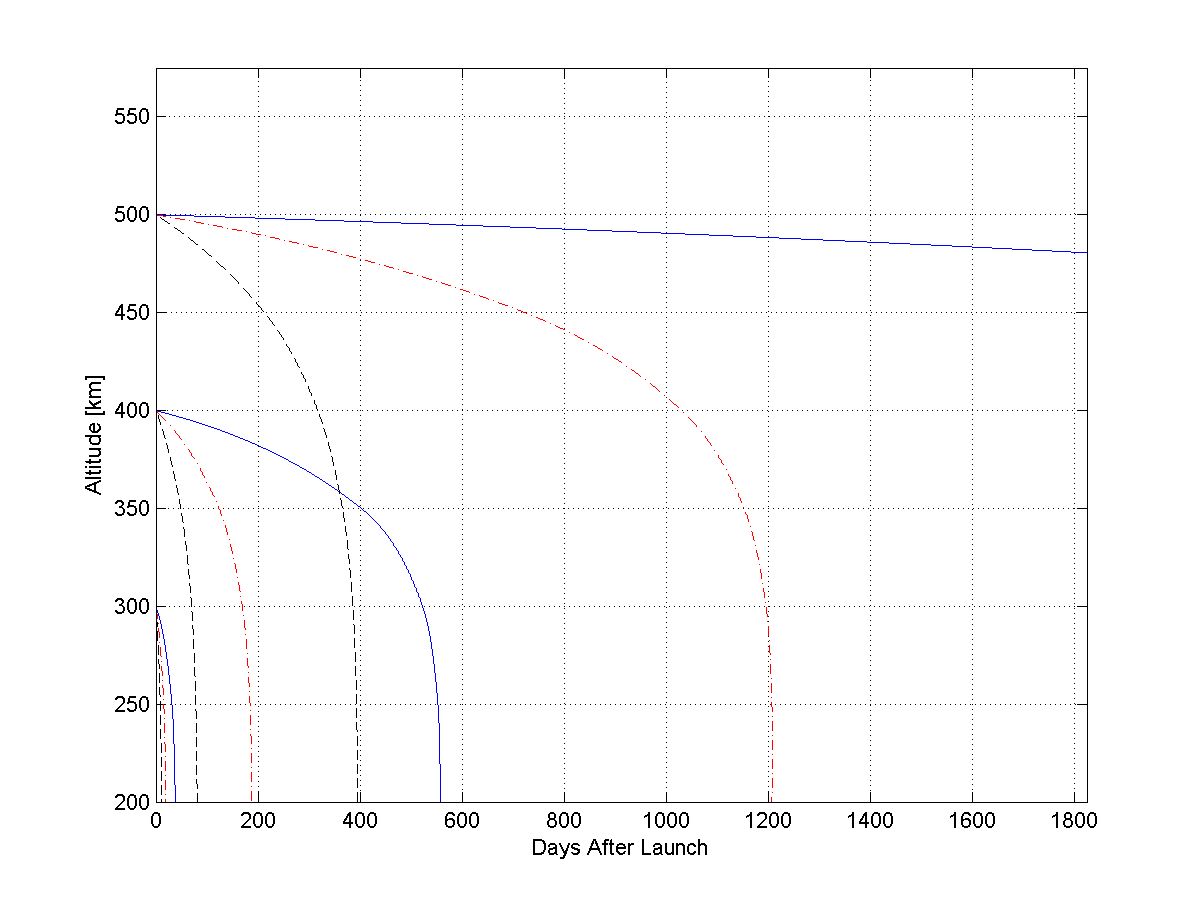
\includegraphics[width=0.95\textheight, angle=90]{img/orbitDecayEmitter.png}
\label{fig:decayEmitter}
\caption{Orbit decay for a satellite with $C_D$ = 4, A = 6.1 $m^2$ and m = 200 kg. Estimates for initial orbital altitudes of 300, 400 and 500 km at solar maximum (- -), solar minimum (--) and time average (-.-) (CHECK MASS AND AREA).}
\end{figure}

\begin{figure}[h!]
\centering
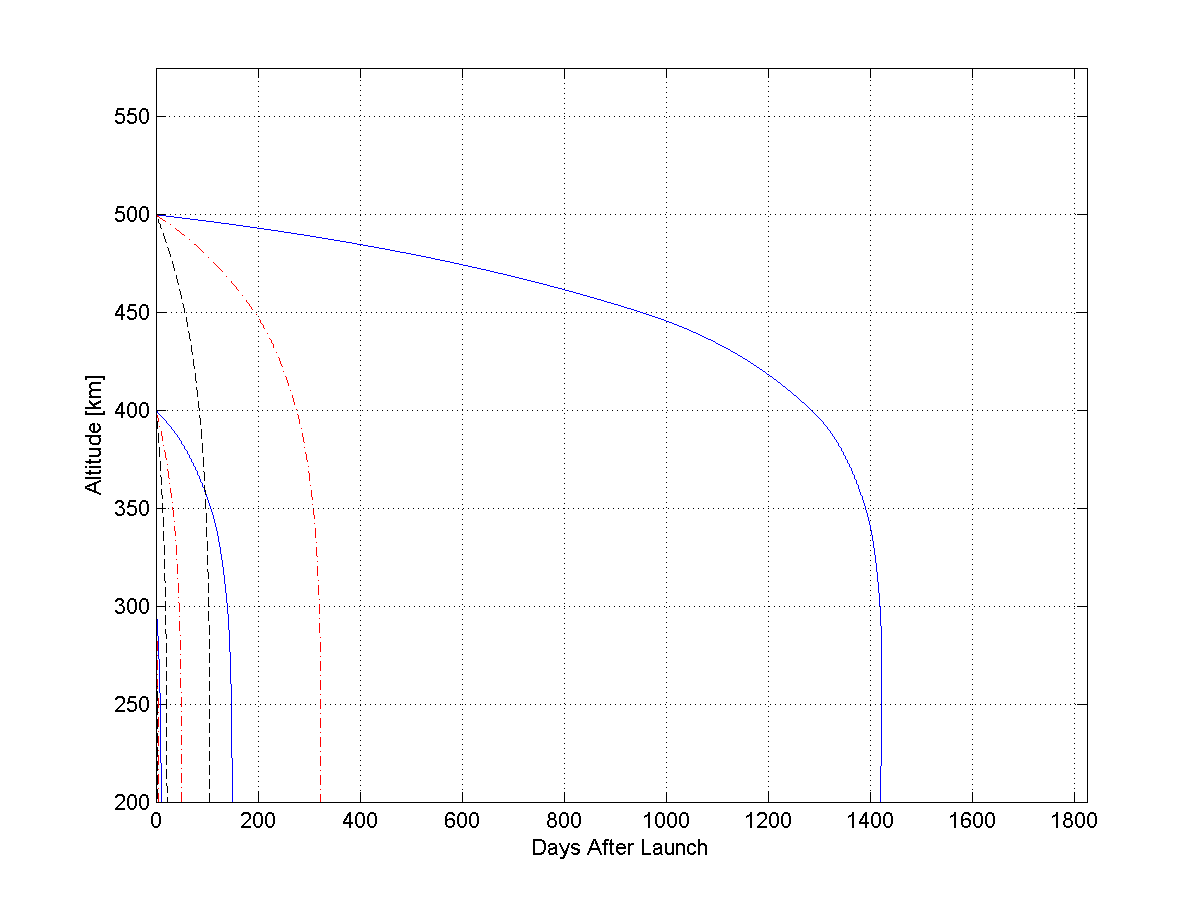
\includegraphics[width=0.95\textheight, angle=90]{img/orbitDecayRecieverMin.png}
\label{fig:decayReceiver}
\caption{Orbit decay for a satellite with $C_D$ = 4, A = 0.21 $m^2$ and m = 10 kg. Estimates for initial orbital altitudes of 300, 400 and 500 km at solar maximum (- -), solar minimum (--) and time average (-.-) (CHECK MASS AND AREA).}
\end{figure}

From the analysis of the orbit decay it is strikingly obvious how important the solar activity is during mission lifetime. Even at an altitude of 500 km neither satellite would be able to maintain its orbit for more then a 100 days (REVISE WITHE AREA NUMBERS). From this analysis it is clear that substantial orbit maintenance is required as the satellites will most probably not have refocusing equipment for the optical instruments. A more comprehensive idea of the orbit maintenance can be gathered from total $\Delta$V estimations shown in figures \ref{fig:deltaVGraph1} and \ref{fig:deltaVGraph2} (pages \pageref{fig:deltaVGraph1} and \pageref{fig:deltaVGraph2}) and tabulated in table \ref{table:deltaVTable} on page \pageref{table:deltaVTable}(CHECK TABLE). This is the total velocity change required to keep the satellites in a certain circular orbit. The calculations are based on equation \ref{deltaV}.

\begin{table}
\centering
\begin{tabular}{ c | c | c | c | c | c | c | c | c | c }
& \multicolumn{3}{|c|}{SOLAR MIN}&\multicolumn{3}{|c|}{TIME AVERAGE}&\multicolumn{3}{|c}{SOLAR MAX} \\ \cline{2-10}
Altitude & 300 & 400 & 500 & 300 & 400 & 500 & 300 & 400 & 500 \\ \hline \hline
EMITTER & 3240.95 & 285.39 & 34.50 & 7716.55 & 1060.48 & 187.88 & 15670.53 & 2943.61 & 691.58 \\
RECEIVER& 2883.54 & 253.92 & 30.70 & 6865.56 & 943.53 & 167.16 & 13942.38 & 2618.99 & 615.32 \\
\end{tabular}
\caption{Required $\Delta$V for various orbit altitudes for a 5 year mission. In $m/s$.}
\label{table:deltaVTable}
\end{table}


It can be clearly seen that $\Delta$V budget is almost five times (CHECK) larger at low altitude at solar maximum when compared to the solar minimum. Overall the values for $\Delta$V at high altitudes, at solar minimum and time average look very favorable. 

\begin{figure}[h!]
\centering
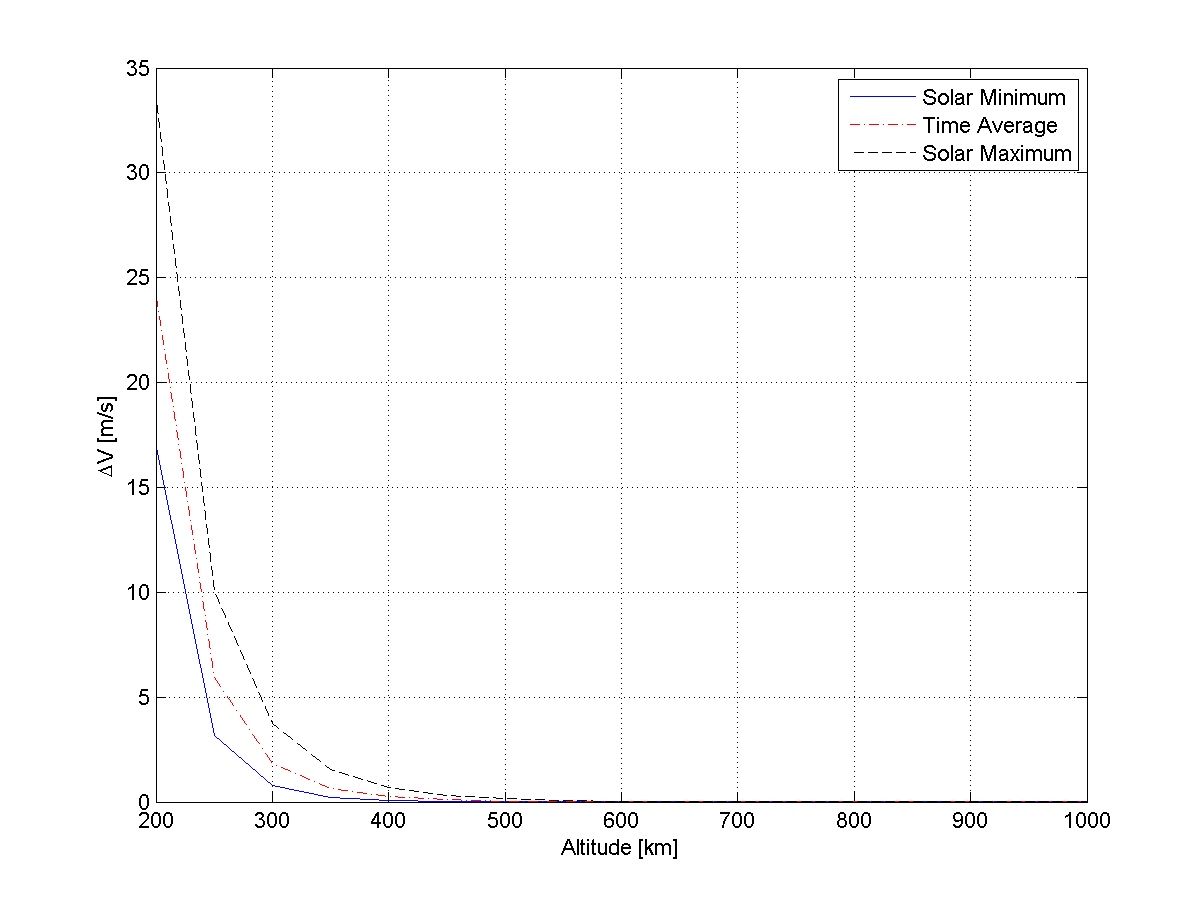
\includegraphics[width=0.95\textheight, angle=90]{img/deltaVEmitter.png}
\label{fig:deltaVGraph1}
\caption{Total $\Delta V$ for a satellite with $C_D$ = 4, A = 6.1 $m^2$ and m = 200 kg. Estimates for a range of orbit altitudes and different solar cycle stages. (CHECK MASS AND AREA).}
\end{figure}

\begin{figure}[h!]
\centering
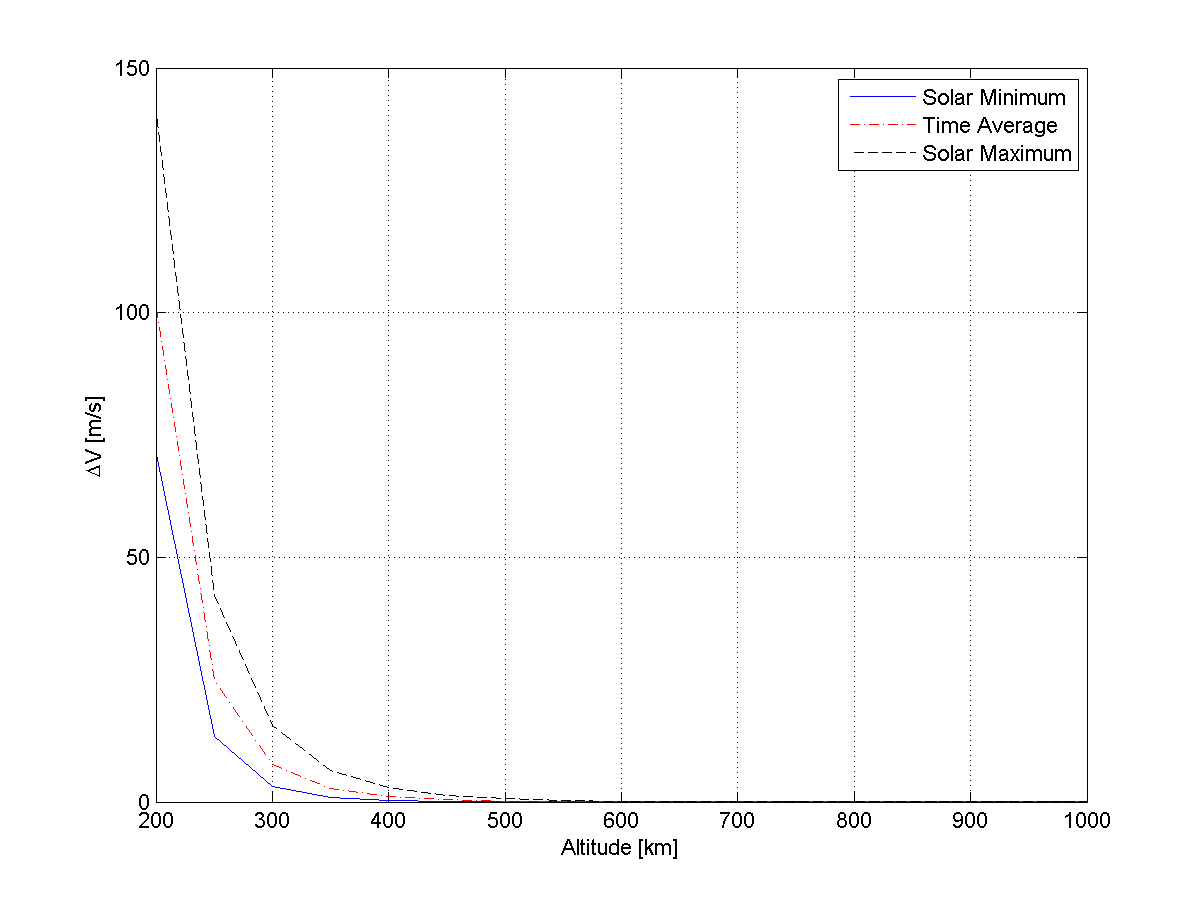
\includegraphics[width=0.95\textheight, angle=90]{img/deltaVReceiver.png}
\label{fig:deltaVGraph2}
\caption{Total $\Delta V$ for a satellite with $C_D$ = 4, A = 0.21 $m^2$ and m = 10 kg. Estimates for a range of orbit altitudes and different solar cycle stages. (CHECK MASS AND AREA).}
\end{figure}   

Three important conclusions can be drawn from the preceding analysis:
\begin{itemize}
	\item In order to avoid fast orbit degradation, and in turn greater mass due to propellant necessary to maintain orbit, the satellites should be placed as high as it is allowable by optical instruments. Based on drag analysis it is recommended to inject at 500 $\pm$ 25 km.
	\item The launch timeframe should be designed in such a way that the mission halftime falls under the solar minimum to reduce drag. This will also allow for a reduction in mass.
	\item The area/mass ratio for the emitter and receiver satellites should be designed as equivalent as possible. This will allow for slower constellation decay and for generally better stationkeeping.  
\end{itemize}
  

\subsection{Exposure to Particle Radiation}
\label{mtrRadiation}

In space, satellites are exposed to streams of highly energetic charged particles coming from the sun. Radiation from these particles can cause severe damage to satellite subsystems, including the payload. The main particle radiation source encountered by the swarm in the \ac{LEO} comes from the Van Allen Belts. These are regions around the Earth where charged particles (protons, electrons and ions) are trapped inside the magnetic field of the planet.

The total radiation dose consists of three components: proton dose, electron dose and the so-called Brehmsstrahlung X-Ray dose produced by the interaction between the electrons and the shielding material of the satellite. In \ac{LEO}, energetic protons in the inner radiation belt contribute most to the total radiation dose. This total is also strongly linked to the orbital altitude and below 1000 km will increase at approximately by the 5\textsuperscript{th} power of the altitude. Furthermore, just like with atmospheric drag, the solar activity plays a major role, thus all cases will be examined.

The number of particles trapped in the Van Allen belts in the vicinity of the orbit under question can be modeled using The Space Environment Information System (SPENVIS) that can be located at the following address: \emph{http://www.spenvis.oma.be/}. SPENVIS contains a large array of NASA and ESA (as well as other) tools and models for complex orbit analysis. For the purposes of this evaluation two models are used: AP-8 and AE-8. The first model predicts proton flux with energy levels above 100 MeV. The latter estimates the flux of electrons with energy of 0.5 MeV or above.

Figure \ref{fig:protFlux} on page \pageref{fig:protFlux} illustrates the trapped proton flux for solar minimum and maximum as a function of distance from Earth Center. It is evident that in \ac{LEO}, the proton flux stays relatively static w.r.t. solar activity. For the considered altitudes of 300 to 500 km (1.047 to 1.078 Earth radii) the satellites would encounter relatively the same order of magnitude of proton radiation. It is also evident that any higher altitude would mean a substantial increase in bombardment and hence reduction in the reliability of the subsystems.   

\begin{figure}
  \centering
  \subfloat[]{\label{fig:protMax}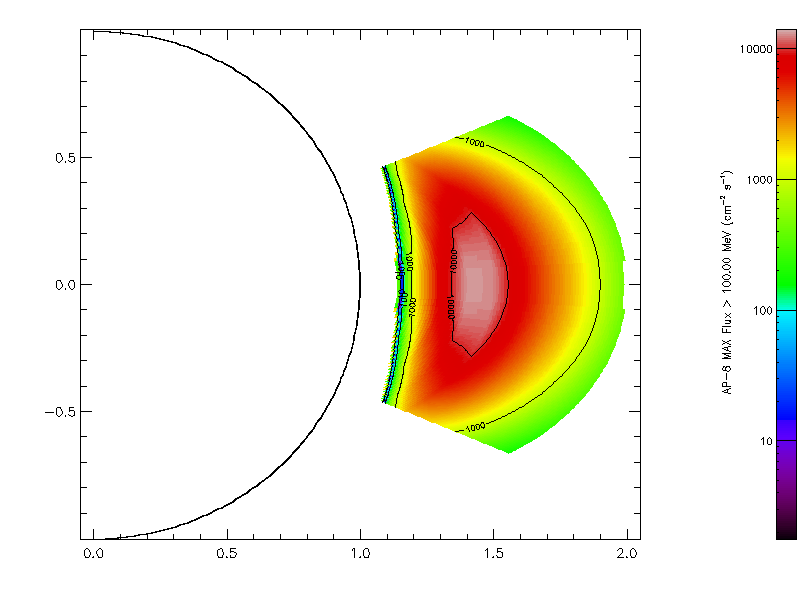
\includegraphics[width=0.7\textwidth]{img/protFluxMax.png}}\\                
  \subfloat[]{\label{fig:protMin}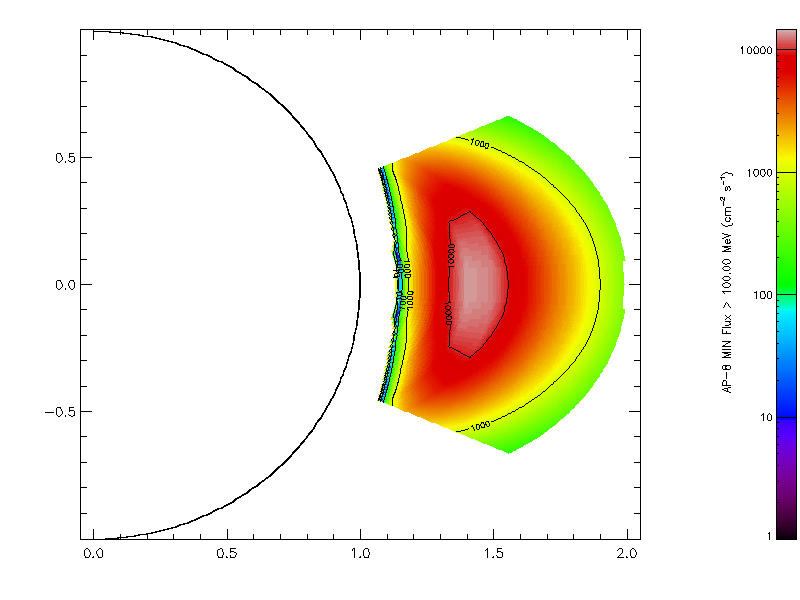
\includegraphics[width=0.7\textwidth]{img/protFluxMin.png}}
  \caption{AP-8 Proton Flux Model (energy $>$ 100 MeV) at solar maximum (a) and solar minimum (b) as a function of distance in mean Earth radii.}
  \label{fig:protFlux}
\end{figure}

Figure \ref{fig:elecFlux} on page \pageref{fig:elecFlux} illustrates the trapped electron flux for solar minimum and maximum as a function of distance from Earth Center. It is evident from this figure that lower altitudes would considerably reduce the radiation flux (up to one order of magnitude).

\begin{figure}
  \centering
  \subfloat[]{\label{fig:elecMax}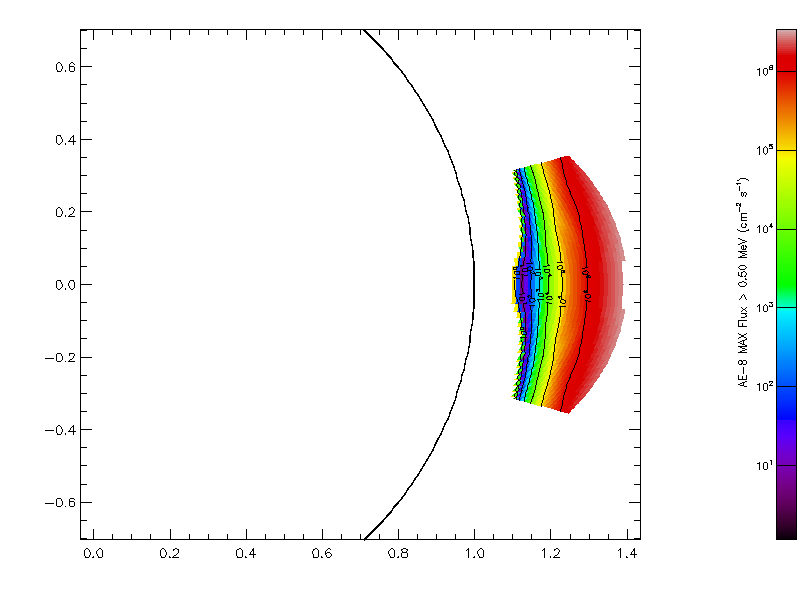
\includegraphics[width=0.7\textwidth]{img/elecFluxMax.png}}\\                
  \subfloat[]{\label{fig:elecMin}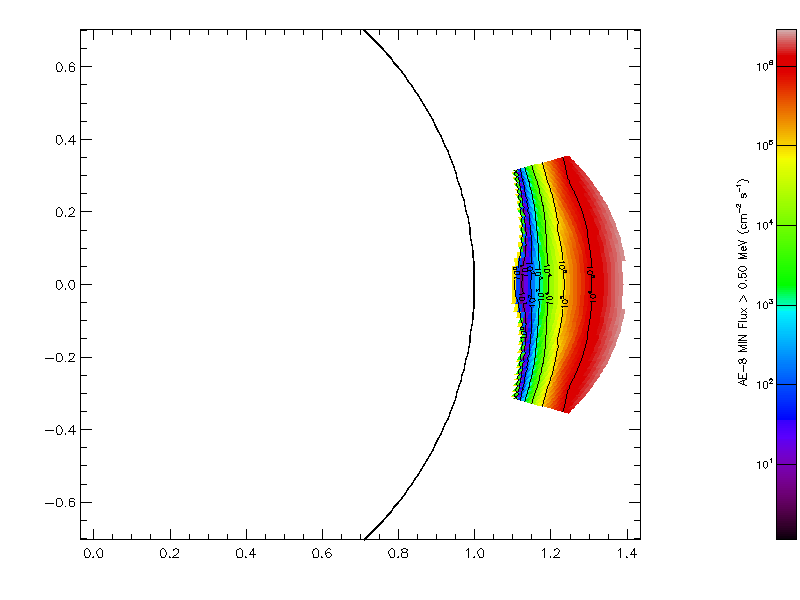
\includegraphics[width=0.7\textwidth]{img/elecFluxMin.png}}
  \caption{AE-8 Electron Flux Model (energy $>$ 0.5 MeV) at solar maximum (a) and solar minimum (b) as a function of distance in mean Earth radii.}
  \label{fig:elecFlux}
\end{figure}

Based on this data, the following conclusion emerges: while altitudes of around 500 km remain relatively safe, a lower orbit will result in a lower particle radiation flux, increasing reliability. Altitudes above 500 km become more and more dangerous for the mission.

\subsection{Conclusion}
\label{mtrAltConclusion}

ADD ALTITUDE CONCLUSION
